\chapter{Исследовательская часть}

В данном разделе будут приведён пример работы программа, а также проведён сравнительный анализ алгоритмов при различных ситуациях на основе полученных данных.

\section{Технические характеристики}

Технические характеристики устройства, на котором выполнялись замеры времени работы реализации алгоритма статической раздачи информации, представлены далее:

\begin{itemize}
	\item операционная система Mac OS Monterey Версия 12.5.1 (21G83) \cite{macos} x86\_64;
	\item память 16 ГБ;
	\item четырёхъядерный процессор Intel Core i7 с тактовой частотой 2,7 ГГц \cite{intel}.
\end{itemize}

При тестировании ноутбук был включен в сеть электропитания. Во время тестирования ноутбук был нагружен только встроенными приложениями окружения, а также системой тестирования.

\section{Демонстрация работы программы}

На рисунке \ref{img:example} представлен результат работы программы.

\img{100mm}{example}{Пример работы программы}
\clearpage

\section{Время выполнения реализаций алгоритмов}

Как было сказано выше, используется функция замера процессорного времени process\_time(...) из библиотеки time на Python. Функция возвращает пользовательское процессорное временя типа float.

Использовать функцию приходится дважды, затем из конечного времени нужно вычесть начальное, чтобы получить результат.

Результаты замеров времени работы реализаций алгоритмов сортировки на различных входных данных (в мс) приведены в таблицах \ref{tbl:best}, \ref{tbl:worth} и \ref{tbl:random}.

\begin{table}[h]
	\begin{center}
		\begin{threeparttable}
		\captionsetup{justification=raggedleft,singlelinecheck=off}
		\caption{Результаты замеров реализаций сортировок, входными данными явллялись отсортированные по возрастанию значений массивы.}
		\label{tbl:best}
		\begin{tabular}{|c|c|c|c|}
			\hline
			Размер & Блинная &  Поразрядная &  Бинарным деревом \\
			\hline
			100 & 0.1662 & 0.0714 & 0.8730 \\ 
			\hline
			200 & 0.5113 & 0.2058 & 3.3267 \\ 
			\hline
			300 & 1.1026 & 0.3131 & 7.6354 \\ 
			\hline
			400 & 2.0140 & 0.4364 & 13.6751 \\ 
			\hline
			500 & 3.3046 & 0.5591 & 21.5524 \\ 
			\hline
			600 & 5.0567 & 0.6798 & 31.3052 \\ 
			\hline
			700 & 6.6944 & 0.7852 & 43.0406 \\ 
			\hline
			800 & 8.5163 & 0.8766 & 56.4318 \\ 
			\hline
		\end{tabular}
		\end{threeparttable}
    \end{center}
\end{table}


\begin{table}[h]
	\begin{center}
		\begin{threeparttable}
		\captionsetup{justification=raggedleft,singlelinecheck=off}
		\caption{Результаты замеров реализаций сортировок, входными данными явллялись отсортированные по убыванию значений массивы.}
		\label{tbl:worth}
		\begin{tabular}{|c|c|c|c|}
			\hline
			Размер & Блинная &  Поразрядная &  Бинарным деревом \\
			\hline
			100 & 0.1606 & 0.1048 & 0.7138 \\ 
			\hline
			200 & 0.5005 & 0.2008 & 2.7633 \\ 
			\hline
			300 & 1.0747 & 0.3110 & 6.3060 \\ 
			\hline
			400 & 1.9383 & 0.4312 & 11.3831 \\ 
			\hline
			500 & 3.1148 & 0.5427 & 18.0577 \\ 
			\hline
			600 & 4.6409 & 0.6693 & 26.0260 \\ 
			\hline
			700 & 6.7969 & 0.8317 & 36.7397 \\ 
			\hline
			800 & 8.7922 & 0.9583 & 47.2628 \\ 
			\hline
		\end{tabular}
		\end{threeparttable}
    \end{center}
\end{table}


\begin{table}[h]
	\begin{center}
		\begin{threeparttable}
		\captionsetup{justification=raggedleft,singlelinecheck=off}
		\caption{Результаты замеров реализаций сортировок, входными данными явллялись заполненные числами со случайными значениями массивы.}
		\label{tbl:random}
		\begin{tabular}{|c|c|c|c|}
			\hline
			 Размер & Блинная &  Поразрядная &  Бинарным деревом \\
			\hline
			100 & 0.2734 & 0.1043 & 0.1560 \\ 
			\hline
			200 & 0.8321 & 0.2090 & 0.3756 \\ 
			\hline
			300 & 1.6837 & 0.3142 & 0.6025 \\ 
			\hline
			400 & 2.8938 & 0.4281 & 0.9785 \\ 
			\hline
			500 & 4.4438 & 0.5419 & 1.1784 \\ 
			\hline
			600 & 6.4153 & 0.6704 & 1.5523 \\ 
			\hline
			700 & 8.6692 & 0.7678 & 1.9018 \\ 
			\hline
			800 & 11.3752 & 0.8992 & 2.2986 \\ 
			\hline
		\end{tabular}
		\end{threeparttable}
    \end{center}
\end{table}

\newpage

Также на рисунках \ref{fig:graph_sorted}, \ref{fig:graph_sorted_back}, \ref{fig:graph_random} приведены графические результаты замеров процессорного времени выполнения реализаций алгоритмов сортировок в зависимости от размера входного массива.

\begin{figure}
	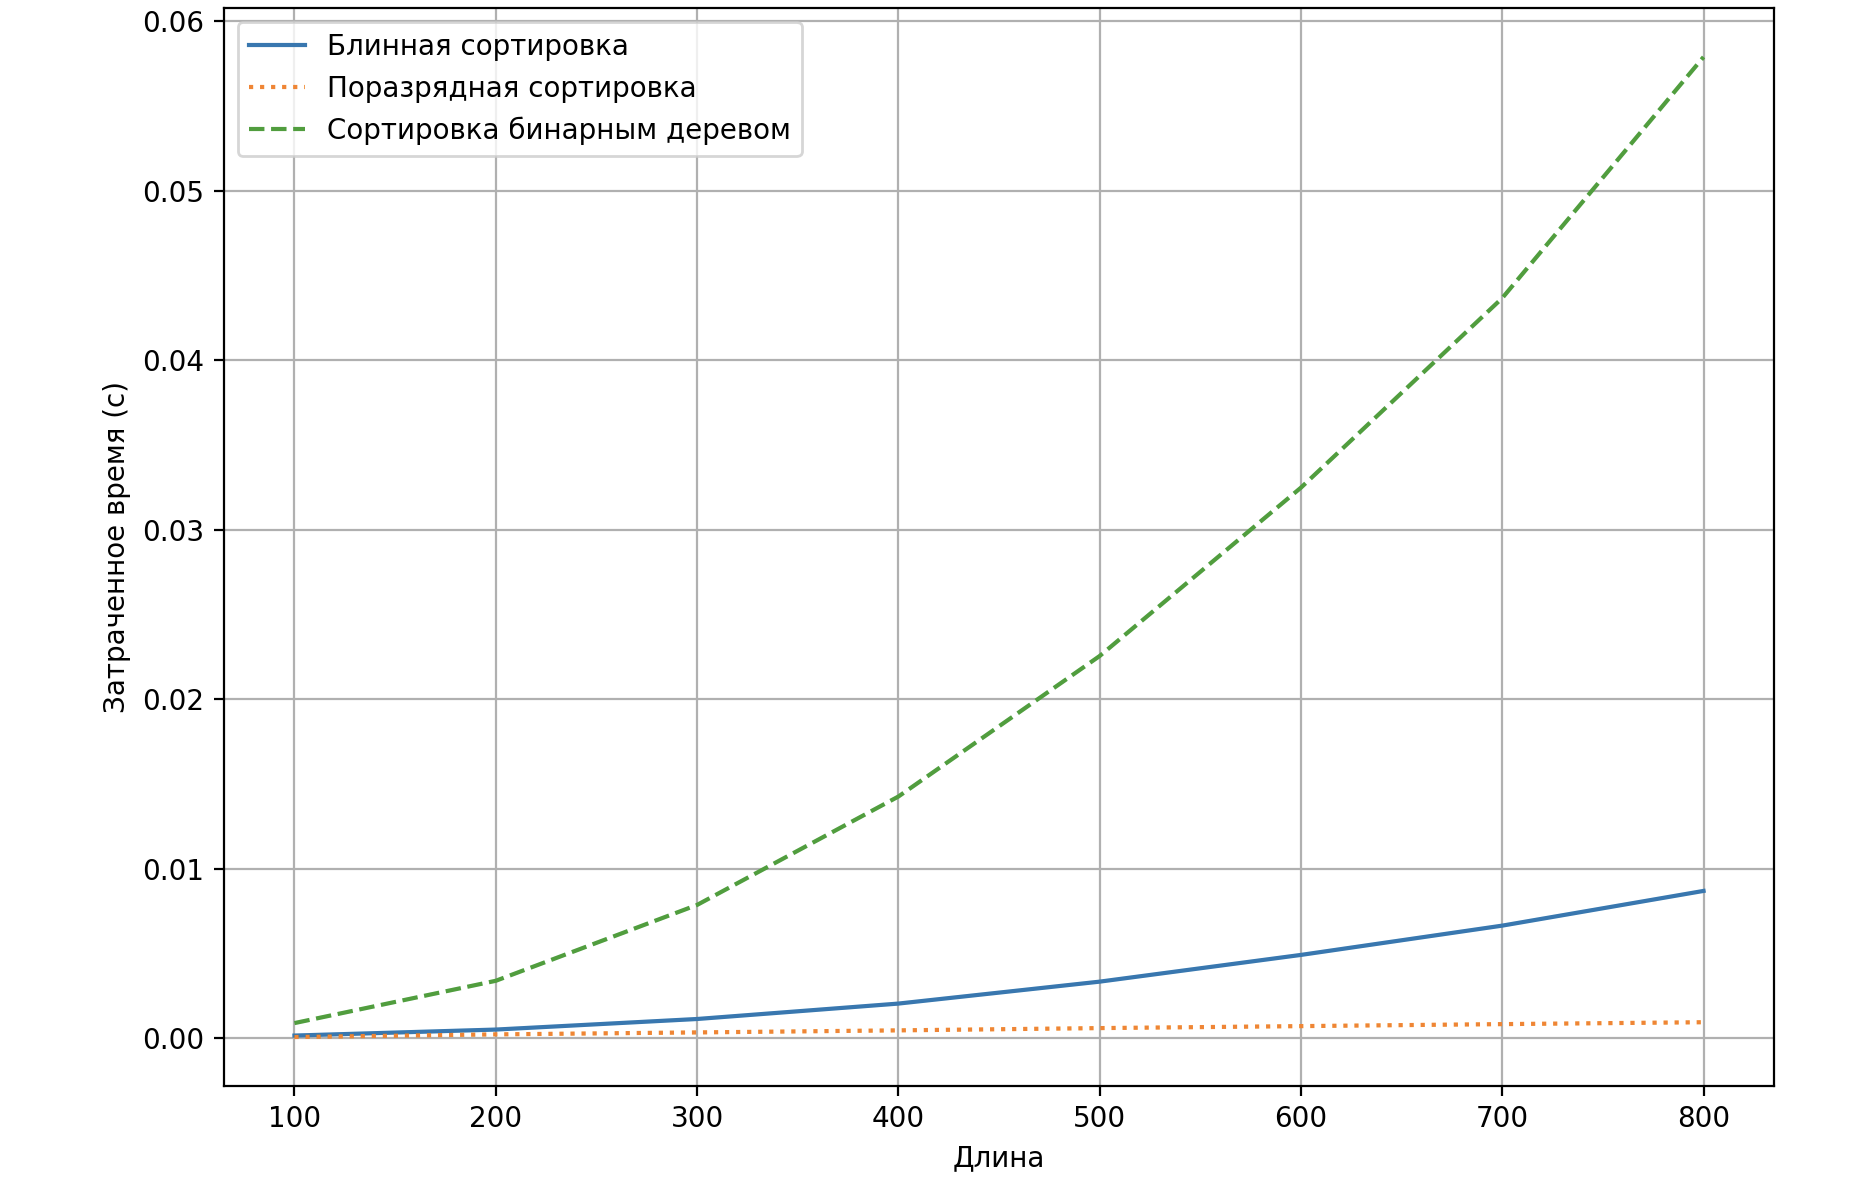
\includegraphics[scale=0.5]{img/graph_sorted}
	\caption{Результаты замеров реализаций сортировок, входными данными явллялись отсортированные по возрастанию значений массивы.}
	\label{fig:graph_sorted}
\end{figure}
\begin{figure}
	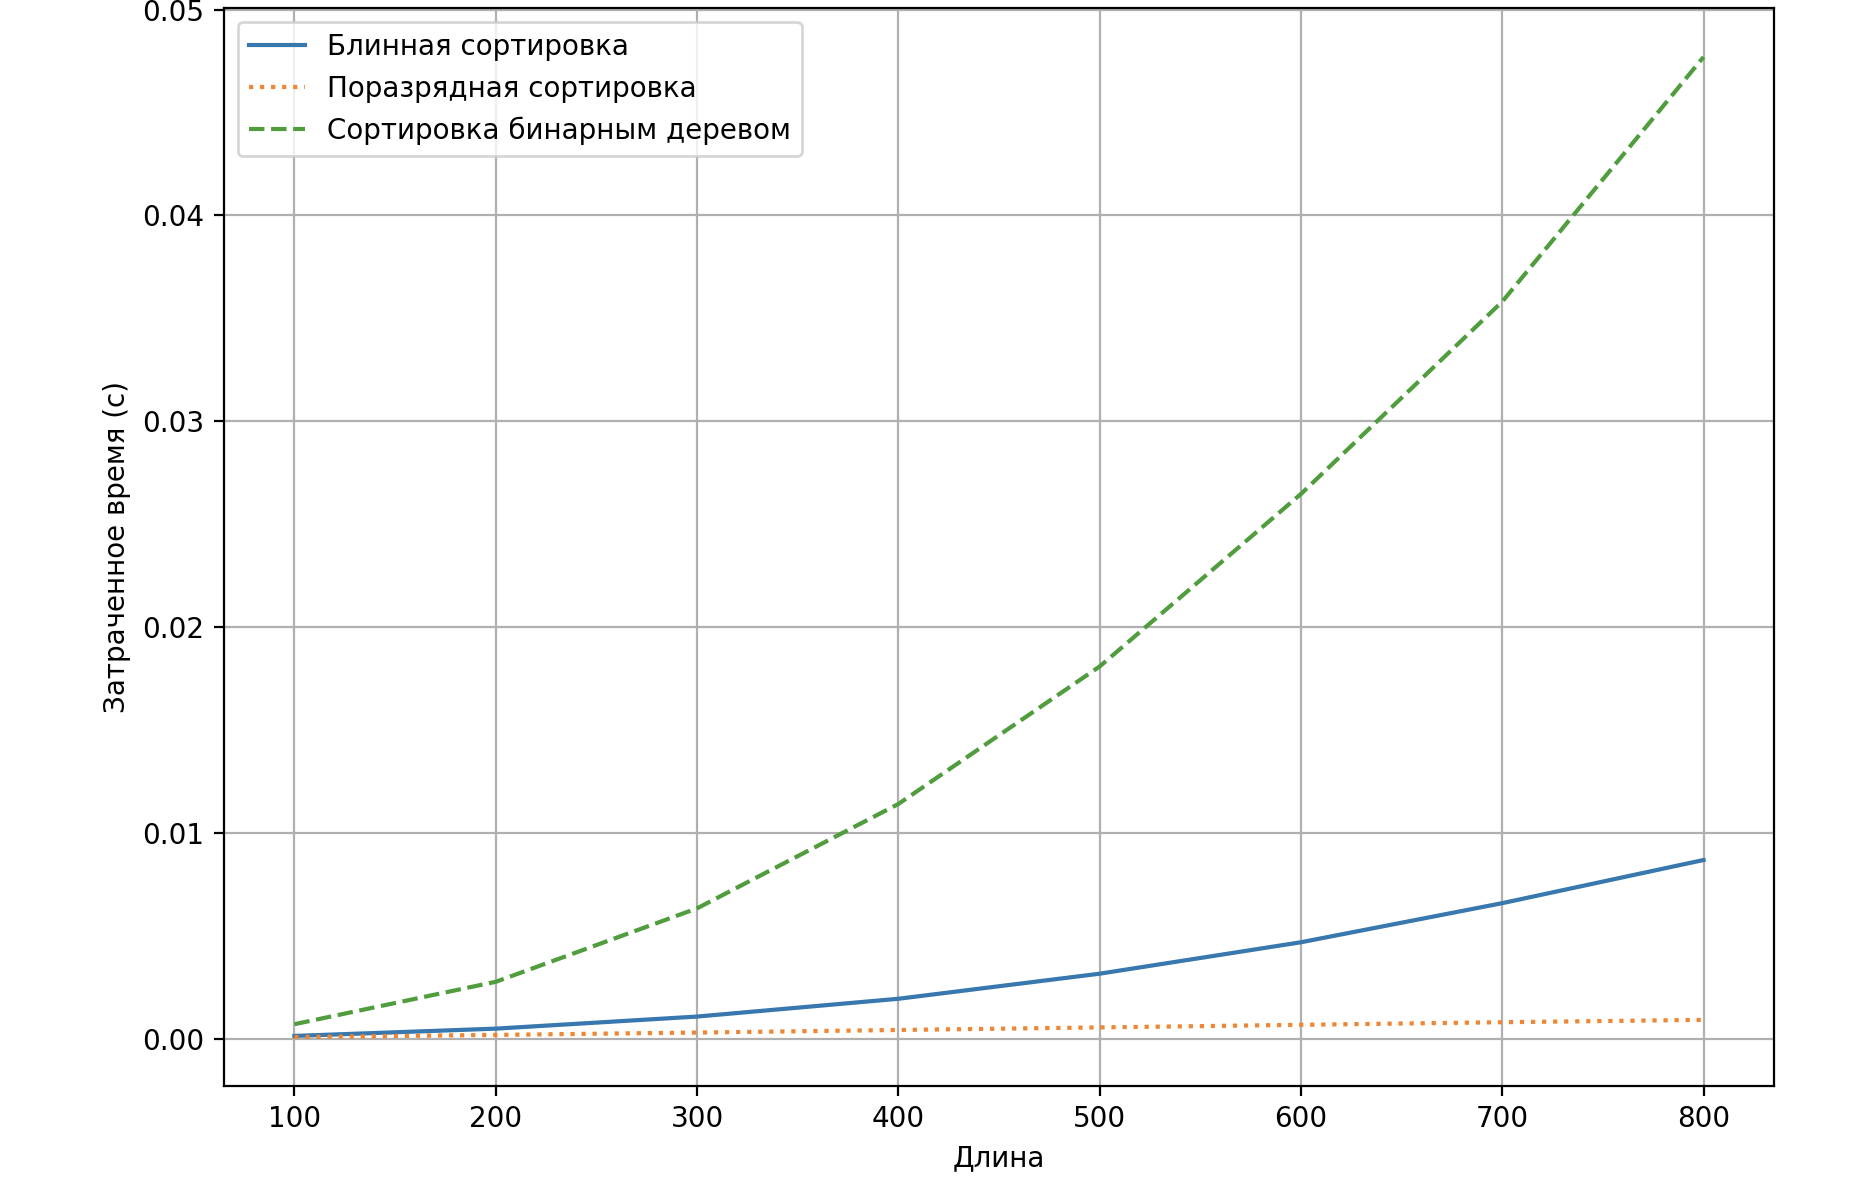
\includegraphics[scale=0.5]{img/graph_sorted_back}
	\caption{Результаты замеров реализаций сортировок, входными данными явллялись отсортированные по убыванию значений массивы.}
	\label{fig:graph_sorted_back}
\end{figure}
\begin{figure}
	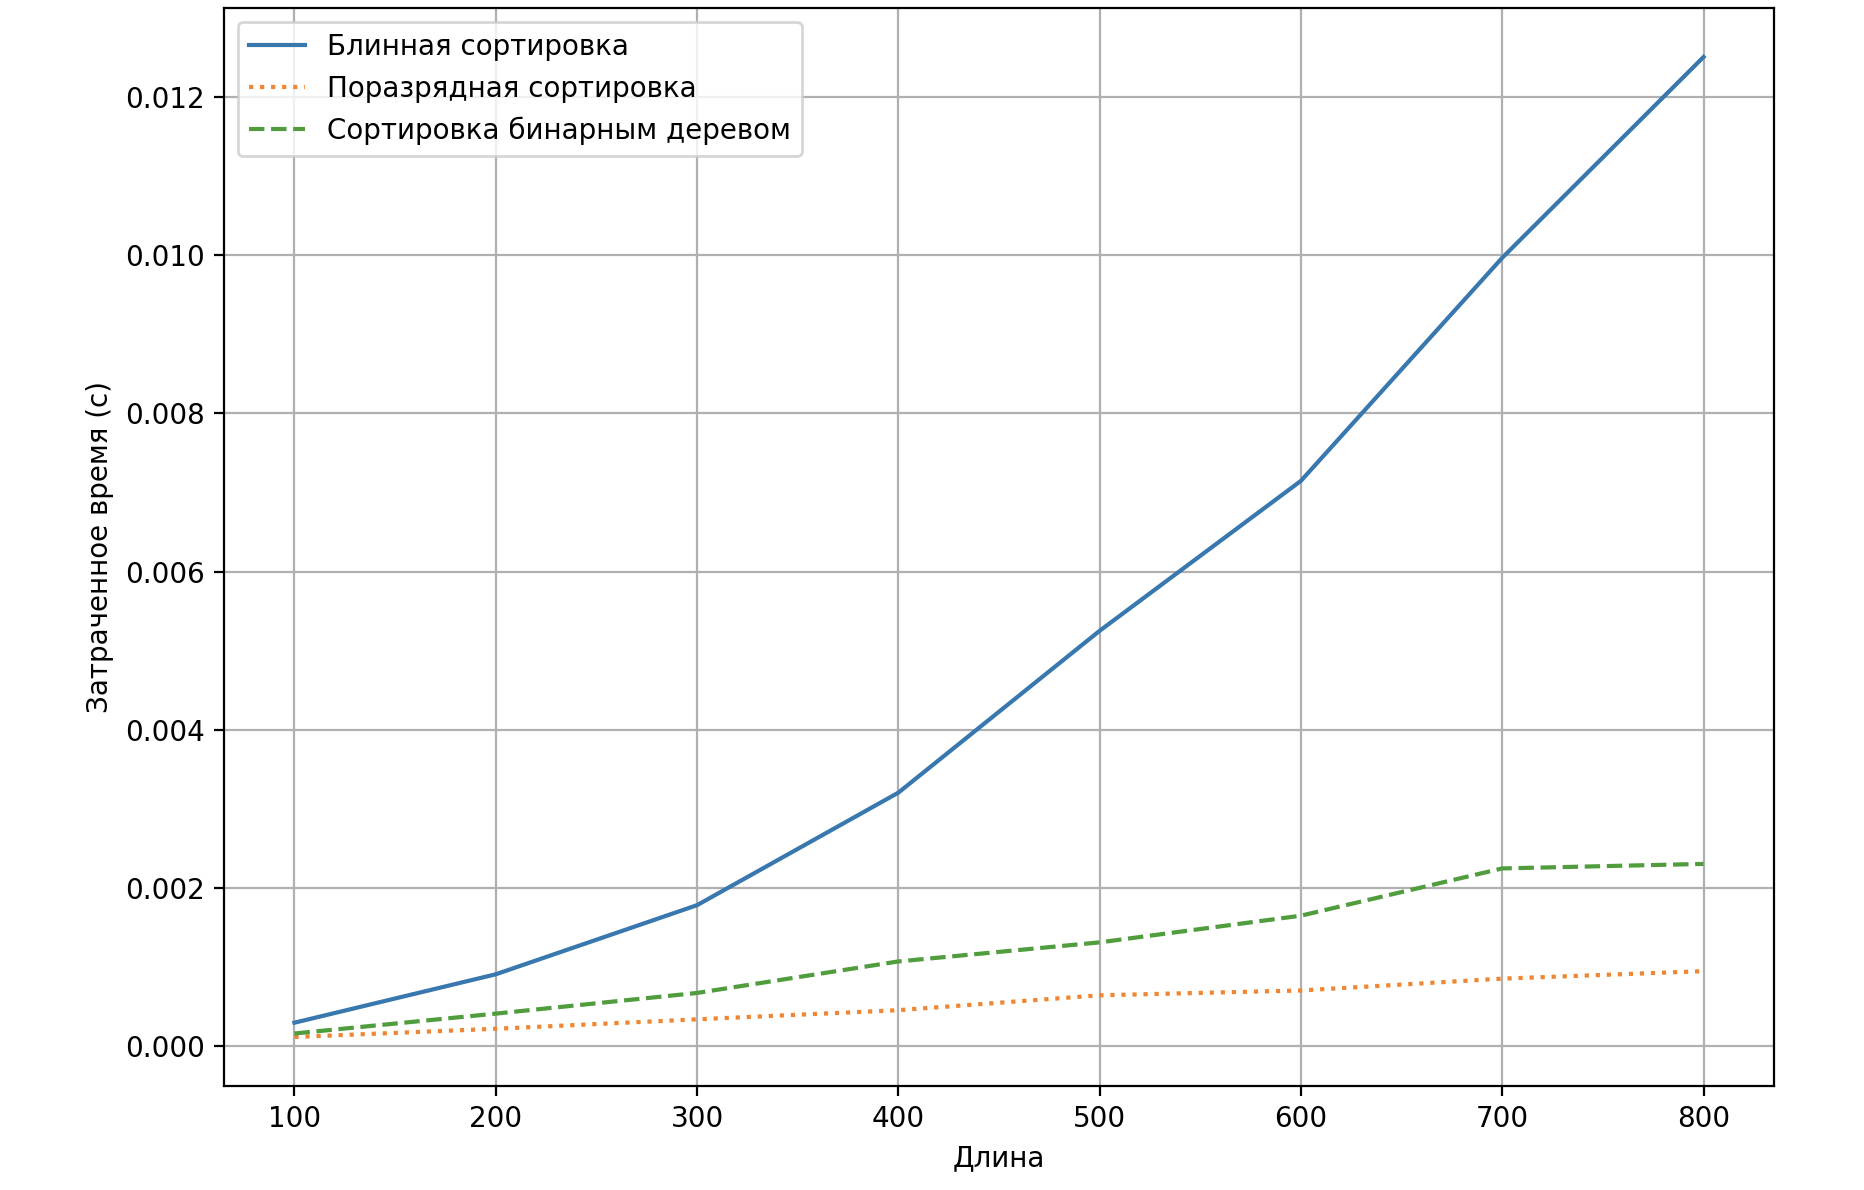
\includegraphics[scale=0.5]{img/graph_random}
	\caption{Результаты замеров реализаций сортировок, входными данными явллялись заполненные числами со случайными значениями массивы.}
	\label{fig:graph_random}
\end{figure}
\clearpage

Сортировка бинарным деревом работает дольше других рассмотренных сортировок на отсортированных масссивах (рисунки \ref{fig:graph_sorted}, \ref{fig:graph_sorted_back}), в то время как на случайно заполненном массиве дольше всех работает блинная сортировка (рисунок \ref{fig:graph_random}). Поразрядная сортировка во всех трёх случаях оказывается самой быстрой.

При этом для блинной сортировки и для сортировки бинарным деревом худшим случаем является подача на вход отсортированного в противоположном поставленному направлению массива, а лучшим -- отсортированного в поставленном направлении. У пораздрядной сортировки нет худших и лучших случаев нет.

\section*{Вывод}
Исходя из полученных результатов, сортировка бинарным деревом на отсортированных массивах и блинная сортировка на случайном массиве работают дольше всех (на длине массива в 800 элементов примерно в 40 раз дольше, чем поразрядная сортировка), при этом поразрядная сортировка показала себя лучше всех на любых данных. Можно сделать вывод, что использование сортировки бинарным деревом показывает наилучший результат при случайных, никак не отсортированных данных, т.к. при отсортированных данных обычное бинарное дерево вырождается в связный список, из-за чего вырастает высота дерева. Поразрядная сортировка же эффективнее в том случае, когда заранее известно максимальное количество разрядов в сортируемых данных.

Теоретические результаты оценки трудоёмкости и полученные практическим образом результаты замеров совпадают.